\subsection{Acapulco (Japanese)}
\vspace{-7.5mm}
\hspace{54mm}
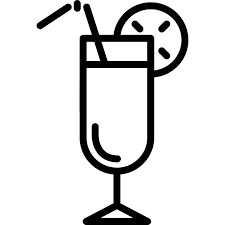
\includegraphics[scale=.07]{cocktail_glass_tall.png}
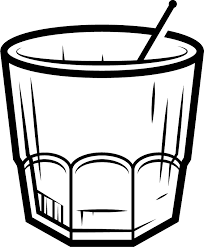
\includegraphics[scale=.06]{cocktail_glass_rock.png}
\vspace{2.5mm}
\begin{itembox}[l]{\boldmath $\reci$}
\begin{itemize}
\setlength{\parskip}{0cm}
\setlength{\itemsep}{0cm}
\item \rum 40ml
\item \cointreau 10ml
\item \lj 10ml
\item \sugar (or \gumsyrup) 1tsp
\item \ew half (optional)
\end{itemize}
\vspace{-4mm}
Made by \shake
\end{itembox}
%There are a lot of variants with a specific name ``Daiquiri''.
Cointreau gives characteristic flavor and body.
The name is from a resort of the south area of Mexico.
